\normaltrue \difficilefalse \tdifficilefalse
\correctiontrue

%\UPSTIidClasse{11} % 11 sup, 12 spé
%\newcommand{\UPSTIidClasse}{12}

\exer{Train simple $\star$ \label{CIN:03:C2:06:26}}

\textit{D'après Florestan Mathurin.}

\setcounter{question}{0}\marginnote{\xpComp{CIN}{03}}%\UPSTIcompetence[2]{A3-05}
%\UPSTIcompetence[2]{C2-06}
\index{Compétence C2-06}\index{Compétence CIN-03}
\index{Train d'engrenages simple}
\ifcorrection
\else
\marginnote{\textbf{Pas de corrigé pour cet exercice.}}
\fi

\ifprof
\else
On s’intéresse au réducteur équipant la roue arrière motrice et directionnelle d’un chariot élévateur de manutention automoteur à conducteur non porté. 


\textbf{Données }: $z_{27} = \SI{16}{dents}$, $z_{35} = \SI{84}{dents}$, $z_{5} = \SI{14}{dents}$, $z_{11} = \SI{56}{dents}$, $z_{16} = \SI{75}{dents}$. 

%\begin{marginfigure}
%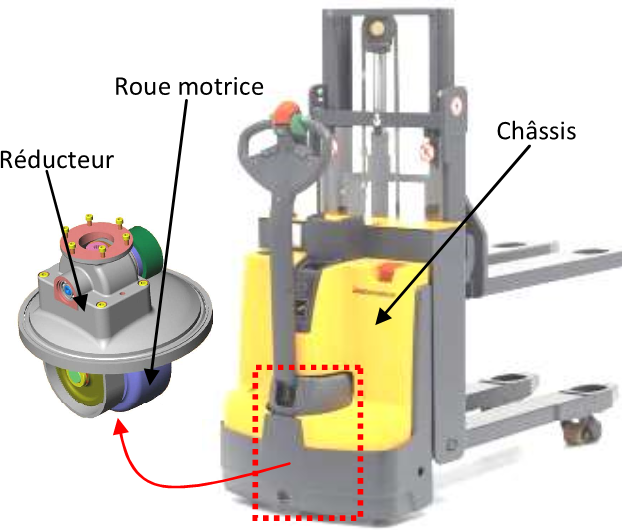
\includegraphics[width=.7\linewidth]{26_01}
%\end{marginfigure}
\fi


\question{Identifier les classes d’équivalence cinématique sur le dessin d’ensemble.}
\ifprof
\else
\begin{marginfigure}
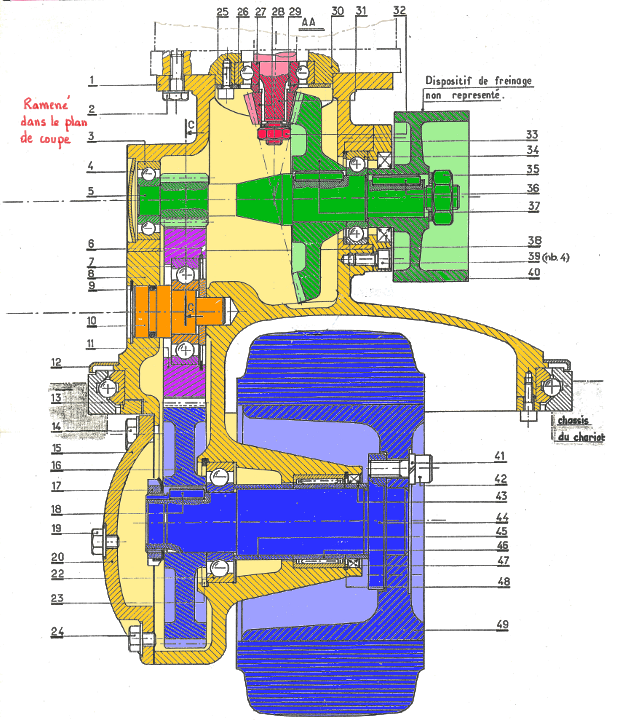
\includegraphics[width=\linewidth]{26_03}
\end{marginfigure}
\fi

\question{ Construire le schéma cinématique du réducteur dans le même plan que le dessin.}
\ifprof ~\\
\begin{marginfigure}
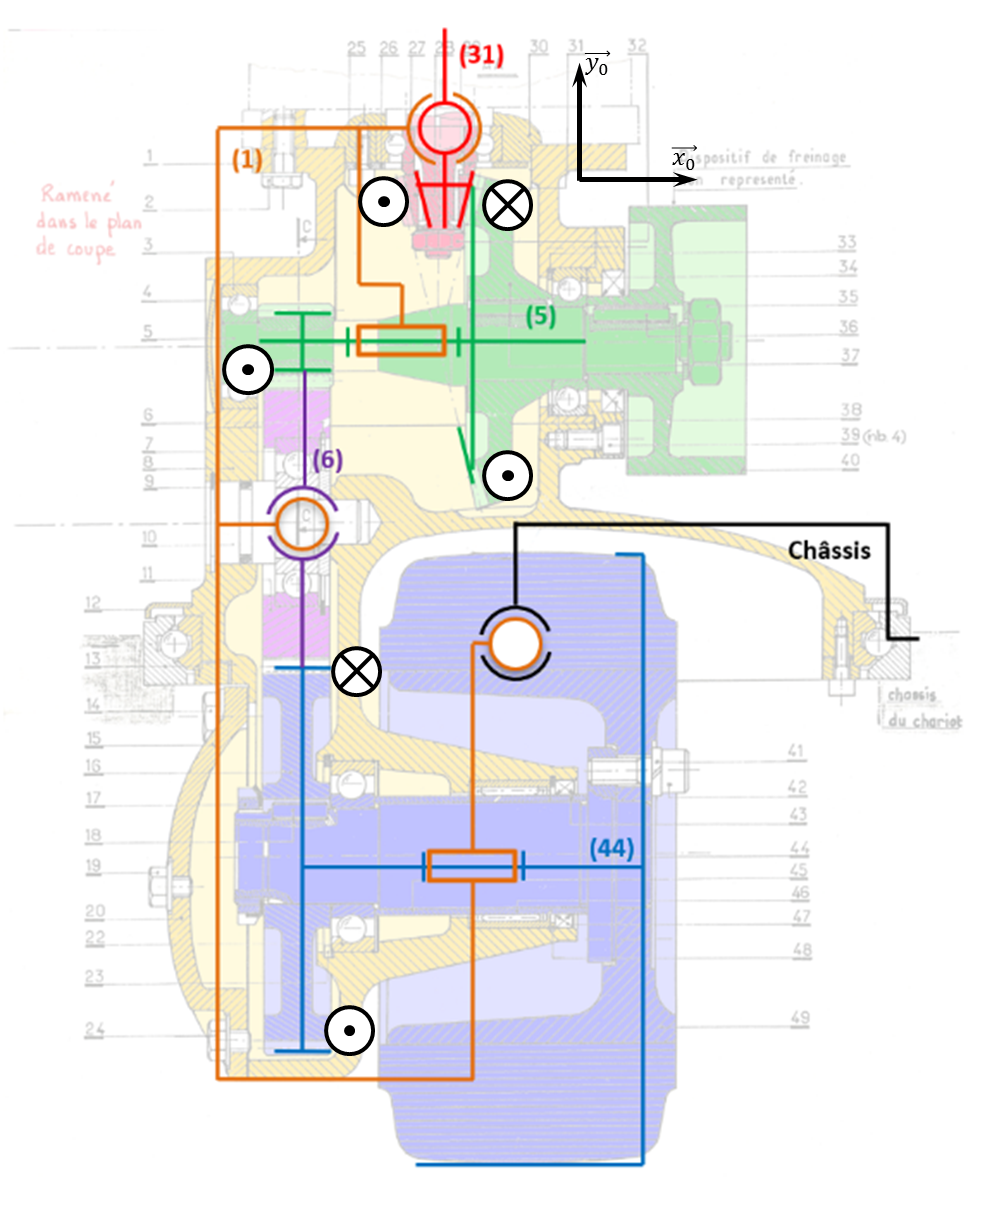
\includegraphics[width=.4\linewidth]{26_cor_01_BIS}
\end{marginfigure}
\else
\fi

\question{Compléter le tableau donnant les caractéristiques des roues et pignons.}
\ifprof

\begin{center}
\begin{tabular}{cccc}
\hline
Repère de  & Module  & Nombre & Diamètre primitif  \\
la roue & $m$ (mm) & de dents $Z$ & $D$ (mm) \\
\hline
27 & 1,5 &16 & 24\\ 
35 & 1,5 &84 & 126\\ 
5   &1,5 &14 & 21\\ 
11 & 1,5 & 56 & 84 \\ 
16 &  1,5&  75& 112,5\\ \hline
\end{tabular}
\end{center}
\else
\begin{center}
\begin{tabular}{llll}
\hline
Repère de la roue & Module  $m$ (mm) & Nombre de dents $Z$& Diamètre primitif $D$ (mm) \\
\hline
27 & & & \\ 
35 & 1,5& & \\
5& & & \\ 
11& 1,5 & & \\ 16& & & \\ \hline
\end{tabular}
\end{center}
\fi


\question{Après avoir proposé un paramétrage, indiquer dans quel sens tourne la roue si le moteur 28 (31) tourne dans le sens positif.}
\ifprof ~\\
Voir figure précédente. Si le moteur tourne dans le sens positif, la roue tourne dans le sens négatif. 
\else
\fi

\question{Pour une vitesse de \SI{1500}{tr/min} en sortie de moteur, déterminer la vitesse de rotation de la roue. Le rayon de la roue est de \SI{150}{mm}. Quelle est la vitesse du véhicule ? }
\ifprof ~\\
Le rapport de réduction de la transmission est le suivant : 
$k=\dfrac{Z_{27} Z_{5} Z_{11} }{Z_{35} Z_{11} Z_{16}} = \dfrac{16\cdot 14}{84\cdot 75} =0,0355 $.

La vitesse de rotation de la roue est donc de $\SI{53,33}{tr.min^{-1}}$ soit \SI{5,59}{rad.s^{-1}}. 
On en déduit la vitesse du véhicule : $5,59 \times 0,15 = \SI{0,84}{m.s^{-1}}\simeq \SI{3}{km.h^{-1}}$.

\else
\fi

\ifprof
\else

\marginnote{Corrigé voir \ref{CIN:03:C2:06:26}.}

\fi